\chapter{Herramientas de Visualización}\label{cap:herramientas_visualizacion}

En el mundo científico, a menudo utilizamos el término \textbf{caja negra} para hacer referencia a sistemas complejos que producen una salida coherente a partir de una entrada dada, pero cuyo funcionamiento interno es difícilmente interpretable o accesible para el observador, como en el caso de las redes neuronales profundas, donde el conocimiento de la red está distribuido en pesos y activaciones de múltiples capas interconectadas.

Por ello, a lo largo del tiempo, se han desarrollado diferentes métodos que nos ayudan a analizar qué ocurre dentro de los modelos, lo que nos permite entender por qué ciertos patrones arquitectónicos funcionan mejor que otros dependiendo del problema, o incluso a ajustar con mayor precisión y de forma más acertada los hiperparámetros del modelo \cite{dl_python__chollet_2021, dl__goodfellow_2016}.

En esta sección se hablará sobre los métodos de visualización más populares en la literatura de redes profundas. Los dividiremos en dos grupos: los que utilizan información del \textit{forward} de la red, como los mapas de características y las activaciones neuronales; y los que se basan en las operaciones con el gradiente en la retropropagación para construir las salidas, como los mapas de saliencia o el Grad-CAM.

\section{Mapas de Características y Activaciones}

Empezando por el más simple, los mapas de características (del inglés, \textit{feature maps}) son las salidas obtenidas al realizar la convolución de la imagen de entrada con cada uno de los filtros de las capas convolucionales de la red. Cada filtro actúa como un \textbf{detector de patrones locales en la entrada}.

\begin{figure}[htb]
	\centering
	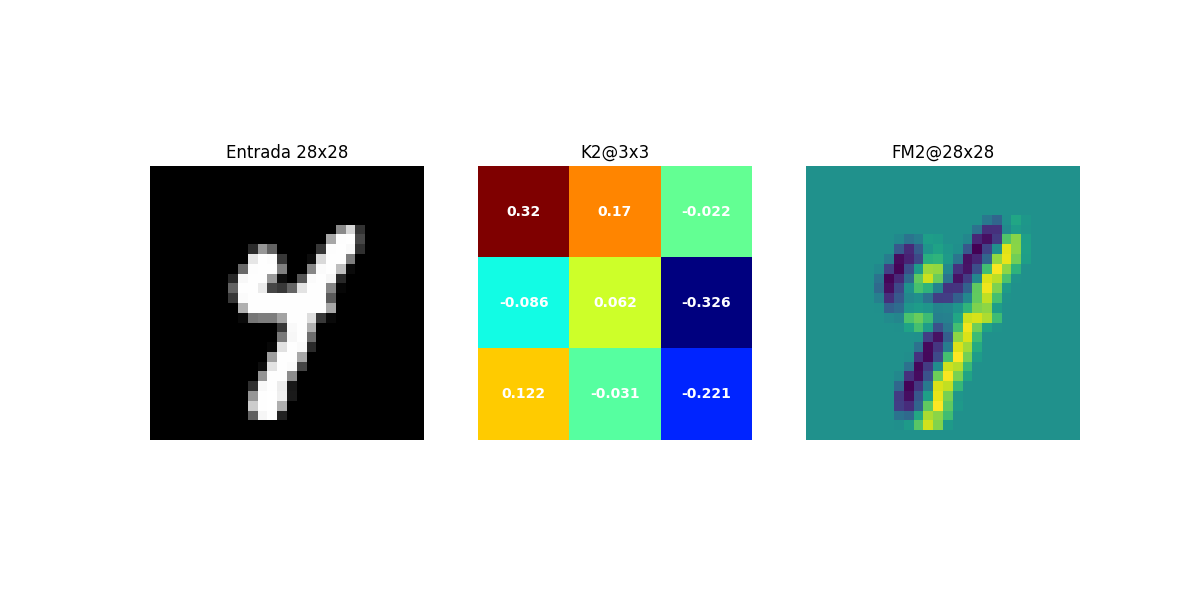
\includegraphics[width=0.7\linewidth]{figures/ejemplos/mapa_caracterisicas_con_kernel.png}
	\caption{Mapa de características obtenido al pasar el kernel K2 de una capa convolucional por una imagen de entrada.}
	\label{fig:mapa_caracterisitcas_kernel_k2}
\end{figure}

En las primeras capas suelen aparecer activaciones que corresponden a \textbf{bordes}, \textbf{esquinas} o \textbf{texturas simples}. Conforme nos adentramos en la red, las activaciones reflejan representaciones cada vez más abstractas: desde contornos y formas como curvas o ángulos, hasta estructuras más complejas, como objetos, en las últimas capas \cite{nn_dl__michael_nielsen_2015}.

Visualizando los mapas de características asociados a una imagen concreta podemos averiguar qué filtros destacan regiones importantes de la imagen, haciéndonos entender fácilmente cómo la red interpreta la información. Por ejemplo, en la figura \ref{fig:convolucion_sobel}, el filtro de sobel aplicado sobre el eje de abscisas de una imagen revela bordes horizontales. Mientras que, sobel aplicado en el eje de ordenadas de una imagen revela bordes verticales.

\paragraph{Activaciones Neuronales}

Mediante la comparación de las activaciones entre diferentes ejemplos, se puede analizar la consistencia de los patrones aprendidos. Si varias imágenes que pertenecen a la misma clase provocan respuestas similares en ciertas neuronas, puede inferirse que dichos nodos codifican características relevantes para esa categoría. Por ejemplo, al introducir un dígito del conjunto MNIST, una neurona de una capa intermedia puede activarse principalmente en presencia de trazos verticales, mientras que otra responde mejor a curvas cerradas \cite{nn_dl__michael_nielsen_2015}.

Estas visualizaciones son especialmente útiles durante la fase de desarrollo, ya que permiten detectar errores en el entrenamiento y ajustar la arquitectura o los hiperparámetros de forma más acertada.

\section{Métodos Basados en el Gradiente}

Los métodos basados en el gradiente ofrecen una forma más precisa de entender qué características concretas de la entrada contribuyen a la decisión final del modelo. A diferencia de las visualizaciones de las activaciones, que muestran qué detecta cada capa, estas técnicas indican qué parte de la entrada causó la activación.

\paragraph{Mapas de Saliencia (Saliency Maps)}
Consisten en calcular la derivada de la salida (por ejemplo, la probabilidad de una clase) con respecto a los píxeles de la entrada (la imagen), obteniendo un mapa de calor cuyos valores de mayor magnitud indican los píxeles más relevantes para la predicción \cite{visualizing__simonyan__2014}. Matemáticamente, consiste en calcular el gradiente de la puntuación de la clase predicha $S_c$ respecto a los píxeles de entrada $I$:

\begin{equation}
	M = \left|\frac{\partial S_c}{\partial I}\right|
\end{equation}

donde cada píxel $M_{ij}$ indica cómo de sensible es la predicción ante un pequeño cambio en el píxel $(i,j)$. En el mapa de saliencia, aquellos píxeles con mayor magnitud corresponden a regiones que influyen más en la clasificación.

\begin{figure}[htb]
	\centering
	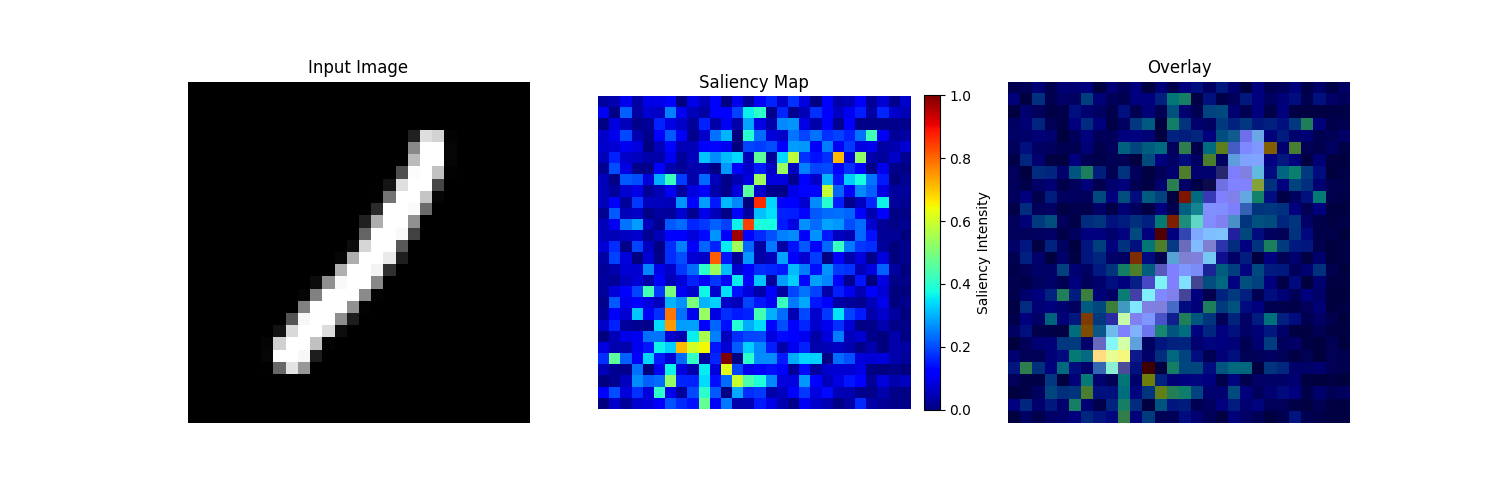
\includegraphics[width=1\linewidth]{figures/ejemplos/saliency_map.png}
	\label{fig:mapa_saliencia}
\end{figure}

Esta técnica fue introducida por \citeauthor{visualizing__simonyan__2014} (\citeyear{visualizing__simonyan__2014}) para redes de clasificación de imágenes \cite{visualizing__simonyan__2014}.

\paragraph{Grad-CAM (Gradient-weighted Class Activation Mapping)}
Grad-CAM Consiste en generar un mapa de calor ponderando los mapas de características de las últimas capas convolucionales con los gradientes asociados a la clase predicha. El resultado es una visualización superpuesta a la imagen original que muestra qué regiones fueron determinantes en la decisión de la red \cite{Selvaraju17-gradcam}.

Estas metodologías son especialmente relevantes en aplicaciones críticas (medicina, conducción autónoma, seguridad), donde es fundamental justificar las decisiones del modelo \cite{examples_nn__kulik_2009, conv_nn_face_recog__chowanda_2019, slam_vehicles__saleem_2023}.

En resumen, las herramientas de visualización permiten comprender mejor qué ocurre en el interior de nuestras redes convolucionales. Gracias a ellas, es posible interpretar qué patrones se aprenden en cada capa y qué partes de la entrada son más influyentes para la predicción.
En el capítulo siguiente se aplicarán algunas de estas técnicas sobre un caso práctico, con el fin de analizar el comportamiento de una red entrenada sobre datos reales.

